\chapter{System Design and Overview}
\label{ch:system_design}
\paragraph{Overview}
 This chapter describes the proposed system from an high level perspective. The purpose of this chapter is indeed to give an overview of how the system modules interact from the point of view of the use cases and data flow analysis. Section~\ref{sec:modelstructure} describes the logical structure of the generative model we use, focusing on the input and outputs and providing the notation we use for the remaining part of this work.
 Section~\ref{sec:usecases} illustrates all the main use cases for the system, highlighting how the different inputs are used to produce the expected results.
 Section~\ref{sec:dataflow} resumes the whole system design focusing on processes and data transformation rather then a component view of the system. 


\section{Generative Model Structure}
\label{sec:modelstructure}
\paragraph{Overview} The initial system design was built upon the architecture of Generative Adversarial Networks \cite{gan} from \citeauthor{gan}. Given the problem of generating video-games levels, the need to control to some extent the generation process naturally arose. For this reason, we adopted a conditional version \cite{conditionalgan} of the GAN Model, proposed by \citeauthor{conditionalgan}, applied to a more recent \gls{gan} model that is discussed in section \ref{sec:networkarch}.


\begin{figure}[h!]
	\begin{center}
		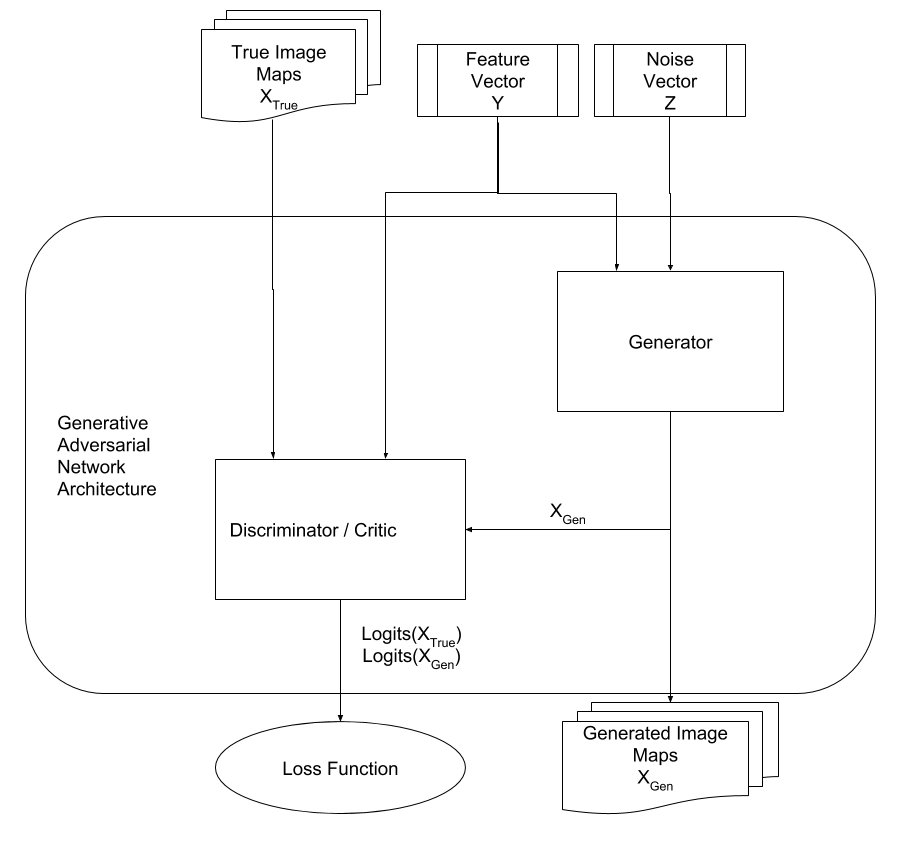
\includegraphics[width=\linewidth]{generative_model_structure}
	\end{center}
	
	\captionsetup{width=\linewidth}
	\caption[System Overview: Generative Model Structure]{ System Overview: Generative Model Structure. A Conditional GAN is composed of a generator model and a discriminative model. The discriminative model takes as input either the Images coming from the dataset or the ones generated by the generative model. Both networks are conditioned by the Y feature vector, while the generator also takes an input a noise vector Z to sample from the data distribution it is approximating. }
	\label{fig:genmodelstructure}
\end{figure}


\paragraph{Conditional GAN Structure} We present in figure \ref{fig:genmodelstructure} the general architecture which defines the inputs and the outputs of the generative model we are using. This structure refers to the Conditional Generative Neural Network we introduced in chapter \ref{sec:introgan}. In particular, figure \ref{fig:genmodelstructure} shows the general working principles of a \gls{gan}: It is composed by two neural networks, namely a Generator and a Discriminator (or Critic, depending on the underlying architecture that is adopted). \\* The input of this subsystem are defined as follows:
\begin{itemize}
	\item $X$: Batch of images having $m$ channels, corresponding to the \glspl{featuremap}.
	\item $Y$: Batch of vectors having one component for each scalar feature considered.
	\item $Z$: Batch of random noise vector, typically sampled from a Uniform or Gaussian distribution.
\end{itemize}

The discriminator network takes as input a vector of images X and a vector of features Y, while the generator network G takes as input a the vector  Y and a vector of random noise Z, which is used to sample different points of the data distribution. We use the subscript "True" or "Gen" to distinguish from the \glspl{featuremap} coming from the input dataset and those that are generated by the generator G.
\\* For what concerns the network outputs, we have that:
\begin{itemize}
	\item  $ X_{Gen} = G(Z|Y) $: Samples generated from the generator network
	\item  $ Logits(X_{Gen}) = D(X_{Gen}|Y) $: Discriminator output when real samples are input to the discriminator.
	\item  $ Logits(X_{True}) = D(X_{True}|Y) $: Discriminator output with generated samples are provided to the discriminator.
\end{itemize}	
Logits are actually the output of the last layer of the discriminator network before the last \textit{activation function}, and they are related to the discriminator assessment of each sample. Loss functions for either the generator and the discriminator are written upon those values and alternately optimized to train the entire network. All the details are given when we'll describe the chosen GAN Architecture and the training process in section \ref{sec:networkarch}.

\section{Use Cases}
\label{sec:usecases}
\paragraph{Overview} This section will describe the main use cases of our system, which are necessary for replicating our results. The emphasis is put on how inputs and outputs are used in each case, while the internal structure of the generative model is not represented in order to simplify the notation. Every figure in this section also describes the function of the dataset metadata introduced in section \ref{sec:metadata_tfrecord} while describing the filtered dataset. In particular the neural network inputs and outputs are limited in a certain range, typically between 0 and 1 or -1 and 1. For this reason, dataset statistics are needed to properly rescale input and output data. Blocks which are written in bold type indicate those inputs and outputs that are of interest for the corresponding use case.

\subsection{Use Case: Model Optimization (Training)}
\label{sec:usecase_train}
\paragraph{} This use case describes the optimization of the model, which is commonly referred as the training phase. This is the phase in which data from the dataset is fed into the model and the loss functions are minimized in order to find the network weights that allow the generation of samples of good quality. In the ideal case the generated samples should come from a distribution which is undistinguishable from the true data distribution. In reality, this is limited by the balance of the discriminator ability in selecting features that allow it to distinguish true data from artificial one, and the generator ability in misleading the discriminator in its task by generating samples that are similar to the real ones. Figure\ref{fig:usecase_train} shows that in this use case both the Scalar Features $Y$ and the Feature Maps $X$ from the dataset are used to train the network. At each epoch the generator network is fed with a random vector $Z$ along with the conditioning vector $Y$. This procedure produces a training loss that is provided to an optimizer that acts on the network weights. 

\begin{figure}[h!]
	\begin{center}
		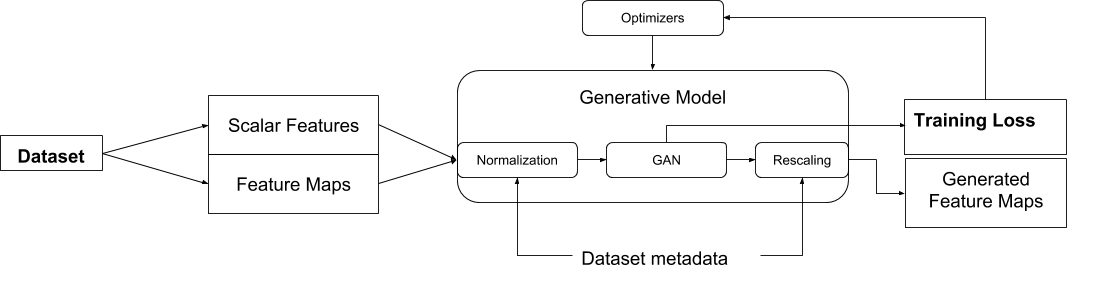
\includegraphics[width=\linewidth]{use_cases_training}
	\end{center}
	
	\captionsetup{width=\linewidth}
	\caption[Use Case: Model Optimization]{Use Case: Model Optimization.}
	\label{fig:usecase_train}
\end{figure}



\subsection{Use Case: Sample Evaluation}
\label{sec:usecase_valid}
\paragraph{} This use case is useful to assess the ability of the model to generate new samples on previously unseen feature vectors and monitoring the training process. This is accomplished by running two different procedures in which only the validation set, composed of samples that are left out from the training phase, is used:
\begin{enumerate}
	\item A \textit{validation loss} is calculated by feeding the discriminator with images $X_{True, Val}$ coming from the validation set and their corresponding feature vector $Y_{Val}$. This approach is often used classical (i.e. discriminative) neural networks, where it is a good method for detecting over-fitting and assessing network generalization capabilities. In our setting, however, this may not always be a meaningful metric with every proposed underlying architecture. This is usually due to the fact that with many \gls{gan} architectures the loss does not correlate well with the quality sample. However, in section \ref{sec:networkarch} we select one of the architectures which propose to reduce the severity of this problem, among others. 
	\item  A set of \textit{quality metrics} (\ref{sec:evaluation}) are computed directly on the true samples $X_{True, Val}$ and the samples $X_{Gen, Val} = G(Z | Y_{Val}) $ generated by conditioning the network with the same features of $X_{True, Val}$. This is based on the assumption that if the network actually learns a correlation between the $Y$ vector of features and a certain set of features proper to the corresponding $X$ samples, then the true sample and the generated one might show a certain grade of similarity according to the given features. Since this may be a strong assumption, especially in the setting where we are not able to measure what features are actually mapped to each component %TODO: Cita un paper che spiega che è difficile mappare il significato delle features nelle GAN
	 $Y_i$ due to the high dimensionality of the problem, a set of more generic metrics are chosen and presented in section (\ref{sec:evaluation}). Selected metrics should be general enough to express, when averaged on batches of samples, a concept of "sample quality" without directly referring to the features encoded in the $Y$ vector.
\end{enumerate}
 Figure~\ref{fig:usecase_valid} shows how the scalar features from the validation set are used to generate new samples, that are compared to the corresponding true images.

\begin{figure}[h!]
	\begin{center}
		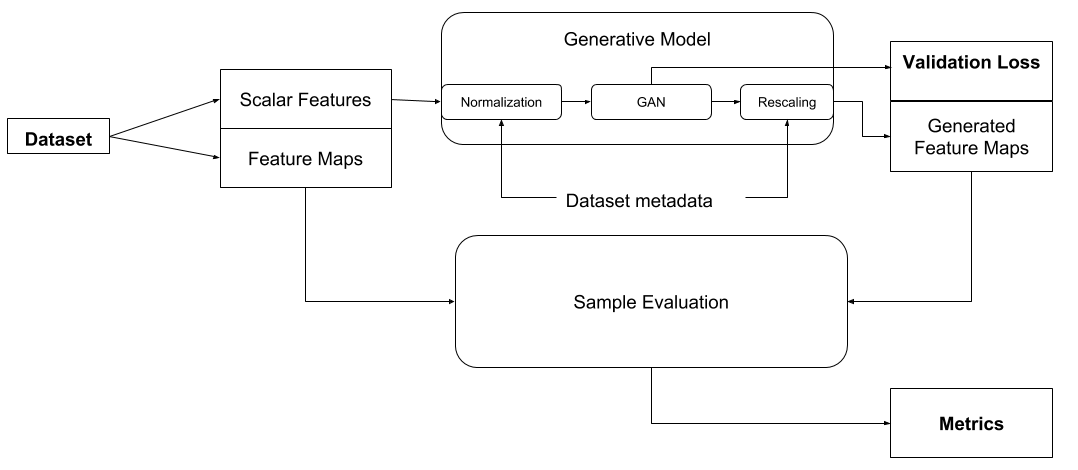
\includegraphics[width=\linewidth]{use_cases_validation}
	\end{center}
	
	\captionsetup{width=\linewidth}
	\caption[Use Case: Validation and Sample Evaluation]{Use Case: Validation and Sample Evaluation.}
	\label{fig:usecase_valid}
\end{figure}

\subsection{Use Case: Sampling or Generation}
\label{sec:usecase_sampling}
\paragraph{} This use case is the one that produces new levels and it is run after a model has been trained. In particular, our system supports several methods for sampling the network in order to generate new levels. \\*
The main problem of sampling this network, as highlighted in the work of \citeauthor{slerp}\cite{slerp}, is choosing a feature vector that has lies in an area that has enough prior probability. We here present four possible methods for sampling our network, while more details are given in section \ref{sec:sampling}. These methods differ, other from the sampling method, on the input that is requested from the user. The noise vector $Z$ can be either random generated for each sampling or kept the same for testing how the $Y$ vector impacts on the network generation.

\begin{itemize}
	\item \textbf{Dataset Sampling}: This sampling method does not require any input from the user, since the conditioning vectors $Y$ are sampled from the dataset.
	\item \textbf{"Factors" Sampling}: This method allows the user to specify a set of scalars $y_{feat} = [y_1, ..., y_f] , y_i \in [0,1]$ where f is the number of features. The extrema correspond to particular values of the related feature, based on the dataset metadata. For example they can match $E[Y_{i}] \pm Std(Y_{i})$ such that each $Y_{i}$ is sampled from a region of the feature space in which it is more likely to have significant probability. This, however, may be not enough because even if the feature components $Y_{i}$ exists in the dataset distribution when taken singularly, this may not hold for their joint distribution. Moreover, the presence of the $Z$ vector greatly increase the dimensionality of the problem. That said, this method can still be useful to easily specify small perturbation in one or more features to inspect the network response, but arbitrary feature sampling remains difficult.
	\item \textbf{Direct Sampling}: This kind of sampling requires the user to directly provide a $Y$ vector as it would come from the dataset. It can be used as a starting point to develop more complex sampling methods.
	\item \textbf{"Content" Sampling}: This kind of sampling is the one that is more interesting from the perspective of an end user. If we consider a design tool that could use this network, we would need to provide the user an interface that is the most natural as possible. Rather than inspecting and "guessing" numerical values, a level designer may be interested in sketching a level and possibly obtaining a set of samples whose features reflect the ones of the provided sketch. We thus propose a sampling method that extracts the feature vector directly from a user generated image, in the same way it is extracted from the \glspl{featuremap} coming from the Dataset.
\end{itemize}
Figure~\ref{fig:usecase_sampling} shows the main differences of the proposed methods in terms of logical transformations and required inputs.

\begin{figure}[h!]
	\begin{center}
		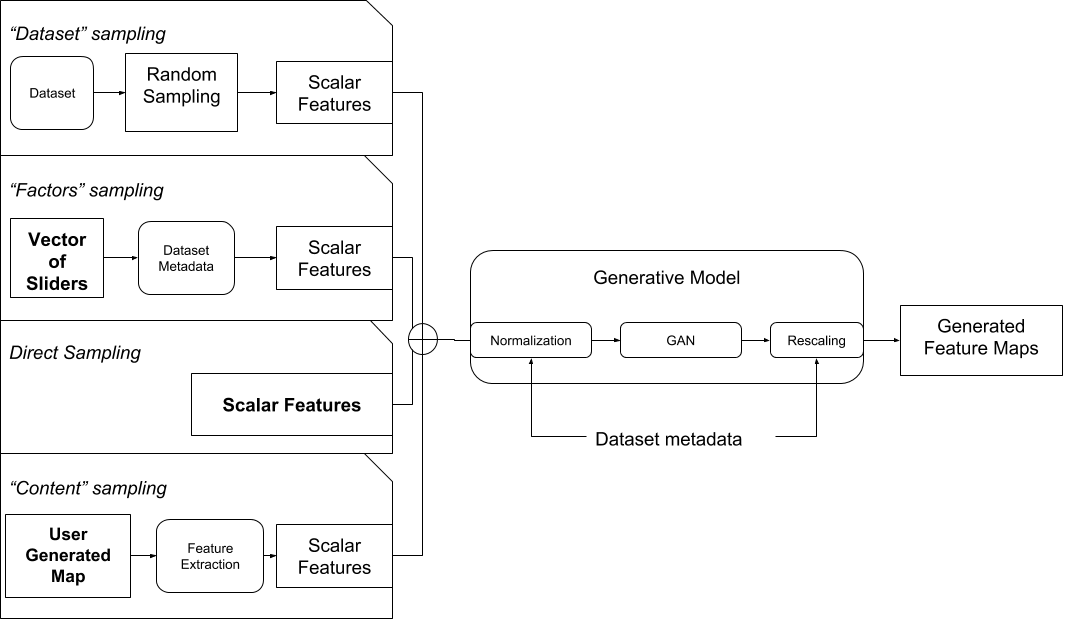
\includegraphics[width=\linewidth]{use_cases_generation}
	\end{center}
	
	\captionsetup{width=\linewidth}
	\caption[Use Case: Sampling or Generation]{Use Case: Sampling or Generation.}
	\label{fig:usecase_sampling}
\end{figure}




\section{Data Flow}
\label{sec:dataflow}
\begin{figure}[h!]
	\begin{center}
		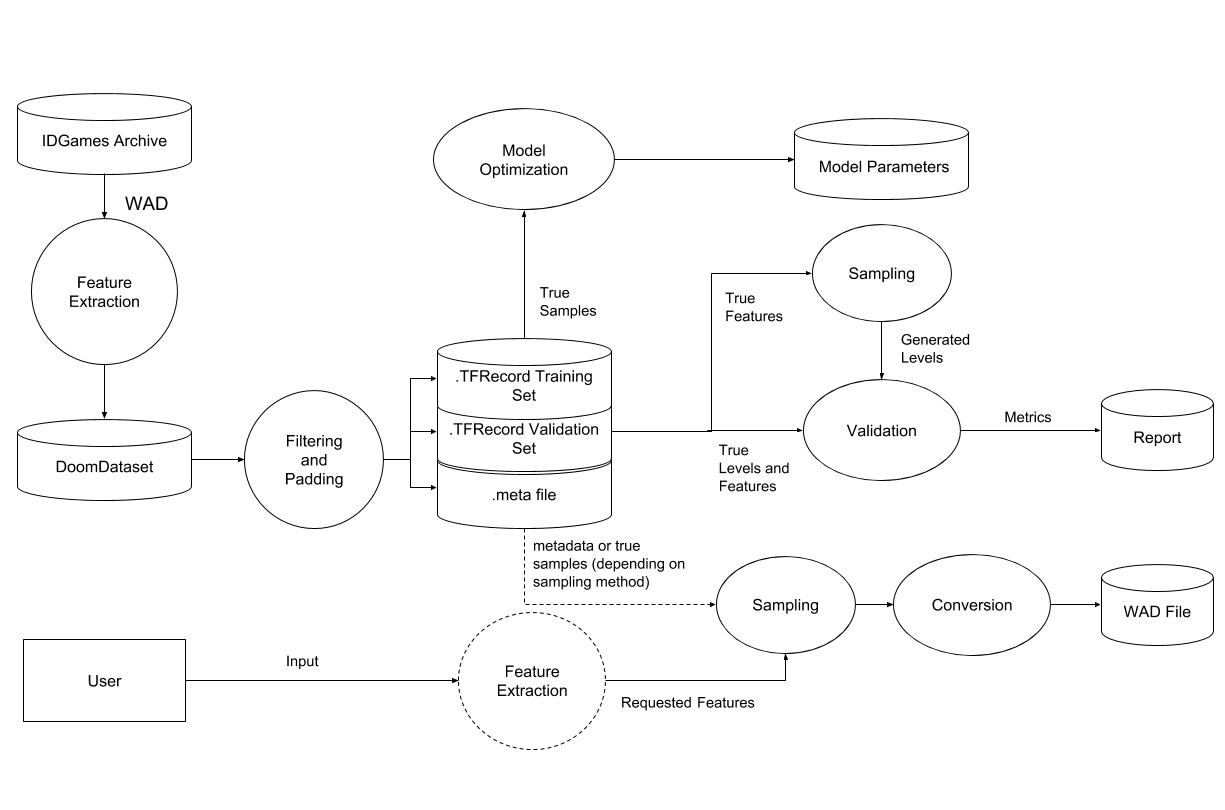
\includegraphics[width=\linewidth]{data_flow_diagram}
	\end{center}
	
	\captionsetup{width=\linewidth}
	\caption[System Overview: Data Flow Diagram]{System Overview: Data Flow Diagram. Disc-shaped blocks represent data archives, circles represent processes and transformations, while the labels on arrows represents intermediate data. Dashed lines represents objects which presence depends on the use case of reference.}
	\label{fig:dataflow}
\end{figure}

\paragraph{} Figure \ref{fig:dataflow} represent the conjunction of the use cases explained in section \ref{sec:usecases}, from a data flow perspective.  The figure is organized as a set of transformations developing from left to right. In particular, blocks on the left represent the inputs to the process and blocks on the right boundary are the produced artefacts. 
It is possible to identify three main data paths: The first produces the model parameters and it is identified with the use case "Model Optimization", or "Training" (\ref{sec:usecase_train}). \\* The second one corresponds to the Sample Evaluation use case (\ref{sec:usecase_valid}) in which levels are generated with a feature vector and then compared with the true ones corresponding to the same feature vector in the dataset. The generated metrics values are stored in a report and showed during the training phase.
The third path, which produces WAD Files, corresponds to the Sampling Use Case (\ref{sec:usecase_sampling}). In this case the data path elements depend on the sampling method used, for this reason they are indicated with dashed lines.

\newpage
\section{WAD Editor and Feature Extractor}
\label{sec:editor}
\paragraph{Overview} In the previous sections of this chapter we described the generative module of the system. The module that remains to be described is the one that copes with the two endpoints of the system, in particular with the conversion from WAD to \glspl{featuremap} (or features) and vice-versa. 
\subsection{Reading and Writing}
\paragraph{Data Collection} As explained in  section~\ref{sec:DatasetOrganization}, data is hosted in an on-line archive. Due to the massive amount of levels a script for automatic download and file extraction has been written. This file also produces a preliminary JSON database, which is further expanded when WAD files are analysed.
\paragraph{Editor} The WAD parser that is provided by \citetitle{VGLC} didn't allow to extract all the features we needed for our data, while other Python modules that offered WAD file access didn't have enough documentation or support or missed features like the ability to create new files. For this reasons we proceeded to write a more complete editor, which offer the user a structured organization of the data that is contained in a WAD file using a more readable format. In particular each WAD file is read as a structured Python dictionary containing all the data we listed in chapter \ref{sec:DatasetOrganization}. The module has been realized so that a developer could ideally build a new map using only a few lines of code or even a PNG Image.


\subsection{Feature Extraction}
\paragraph{Overview} The feature extraction process is built upon our WAD Editor. In particular each WAD is first read as a structured Python dictionary, than it is processed to extract the set of features we provide with the dataset.
\paragraph{WAD to Feature Maps} The process of generating the Feature Maps is quite straightforward: For each \gls{sector} the floor height is drawn as a filled polygon on an image and the sector tags annotated. Then, each linedef is drawn as a straight line, producing the \gls{wallmap}, thus linedef triggers are matched with the relative sector tags for generating the \gls{triggermap}. \glspl{floormap} are derived by simply flattening the heightmap colour. During the process that generates the \glspl{featuremap}, the scalar features are computed on the feature maps themselves or directly from the sector and linedef data, depending on the feature. In this phase, the graph and the textual representation are also produced. 
\paragraph{Feature Maps to WAD} The WAD Editor is also able to produce WAD files from the feature map PNG representation of a level. In principle, it is possible to generate a level by  using a bitmap image editor. A more interesting use, instead, would be using this editor to write the levels generated from the network back to a WAD file, and inspect them directly in game. This is possible, at the cost of a slight loss of information due to the pixel representation of the level. In particular, line detection algorithms such as the Hough transform Line detection algorithm \cite{hough} or its probabilistic version \cite{houghprob} did not work well as expected in detecting walls from the levels generated by the network. Another approach we tried was using an edge detection algorithm for drawing sectors as contours, but this revealed to be too complex due to the way sectors are specified in WAD files (\ref{sec:WAD}). We used an alternative approach instead, exploiting the information provided by the Room Adjacency Graph built upon the \gls{roommap}: For each edge in the graph, which correspond to the boundary between a room and another, a set of walls is defined and their coordinates annotated within the graph. Approximating each sector as an entire room the process of drawing the entire map room-by-room became more straightforward. The work of inserting height changes in parts that are smaller than a room can be done by further segmenting the heightmap when considering each room and it is left as a future work.

\section{Summary} 
% We presented a framework for machine learning based level generation that is general enough to be used at least with any generative adversarial network 
In this chapter we presented a framework that can be used to train generative models, in particular Generative Neural Networks, to produce new levels from a previously collected dataset. In order to cope with the difficulties in sampling the network and evaluating the samples, we presented alternative methods for conditioning the network during the generation phase and for evaluating the generated samples. Moreover, we introduced our module for converting WAD levels into a set of \glspl{featuremap} and vice-versa.